\section{Desarrollo}

\subsection{Introducci\'on}
\begin{frame}
\frametitle{Introducci\'on}

\begin{figure}[h]
\centering
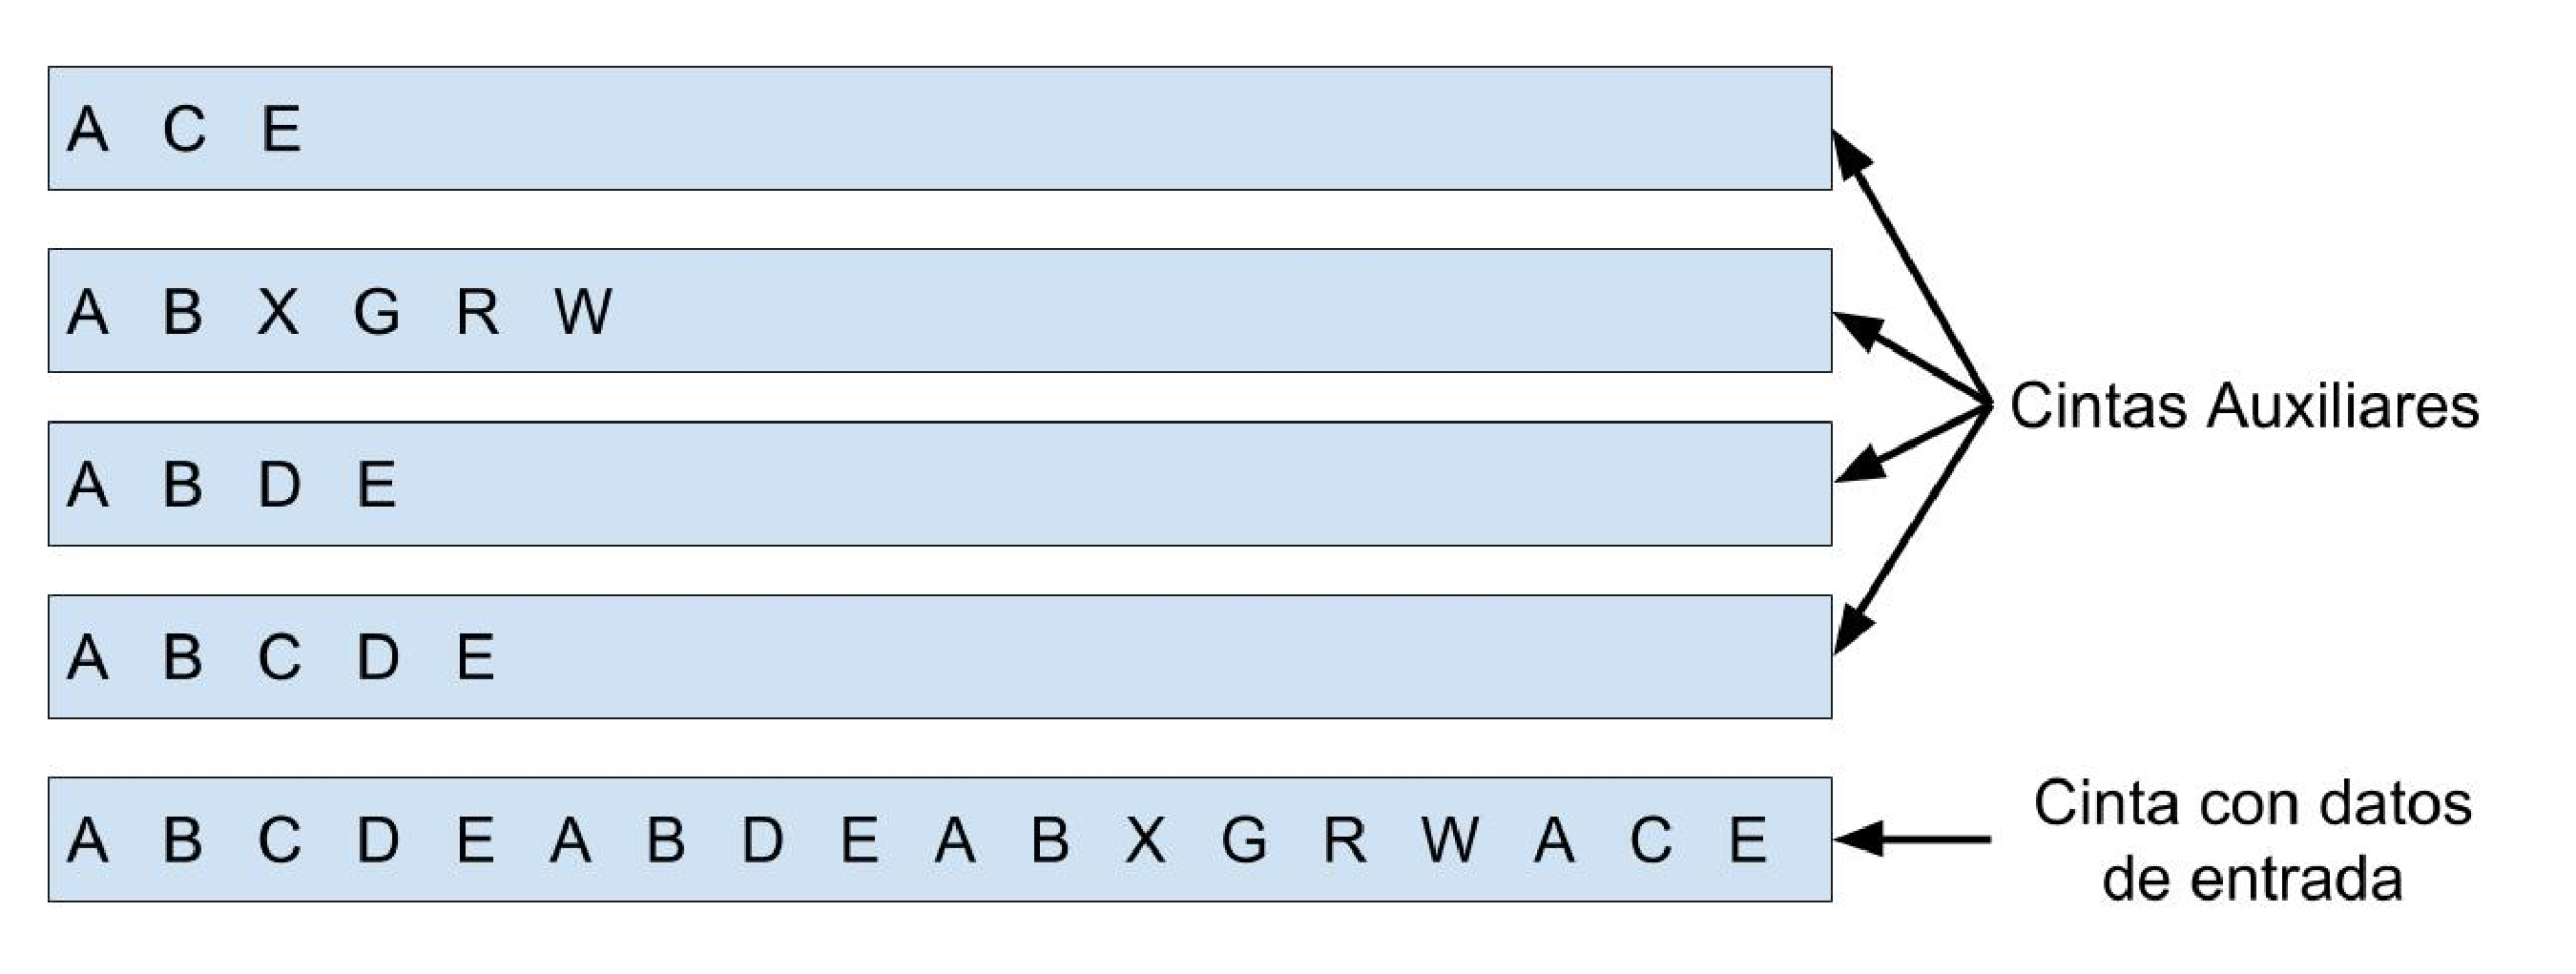
\includegraphics[width=1.0\columnwidth]{Imagenes/algoritmo1.eps}
\caption{Ejemplo del algoritmo con una m\'aquina de Turing multicinta.}
\label{fig:alg01}
\end{figure}

\end{frame}


\begin{frame}
\frametitle{Introducci\'on}

\begin{figure}[h]
\centering
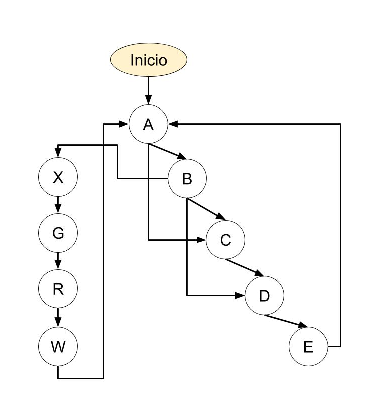
\includegraphics[width=0.5 \columnwidth]{Imagenes/algoritmo2.eps}
\caption{Ejemplo del algoritmo con un grafo dirigido.}
\label{fig:alg02}
\end{figure}

\end{frame}


\subsection{Desarrollo}
\begin{frame}
\frametitle{Vector de caracter\'isticas}

\begin{table}[!h]
\centering
\begin{tabular}{cccc}

\textbf{[Tiempo,} 
& \textbf{Dispositivo,} 
& \textbf{Acci\'on,}
& \textbf{Colocaci\'on]}
\\

& Keyboard
& Pressed
& Key
\\

& Mouse
& Release
& Button
\\

& 
& Scrolled
& Direction
\\

& 
& Moved
& Coordinates(X,Y)
\\


\end{tabular}
\end{table}

\begin{block}{\centering Muestra de acciones capturadas}
\centering
0.06,Mouse,Moved,1028,324\\
0.48,Mouse,Scrolled,Down\\
0.0,Keyboard,Pressed,Key.enter\\
\end{block}

\end{frame}


\begin{frame}
\frametitle{Funcionamiento}
\begin{figure}[H]
\centering
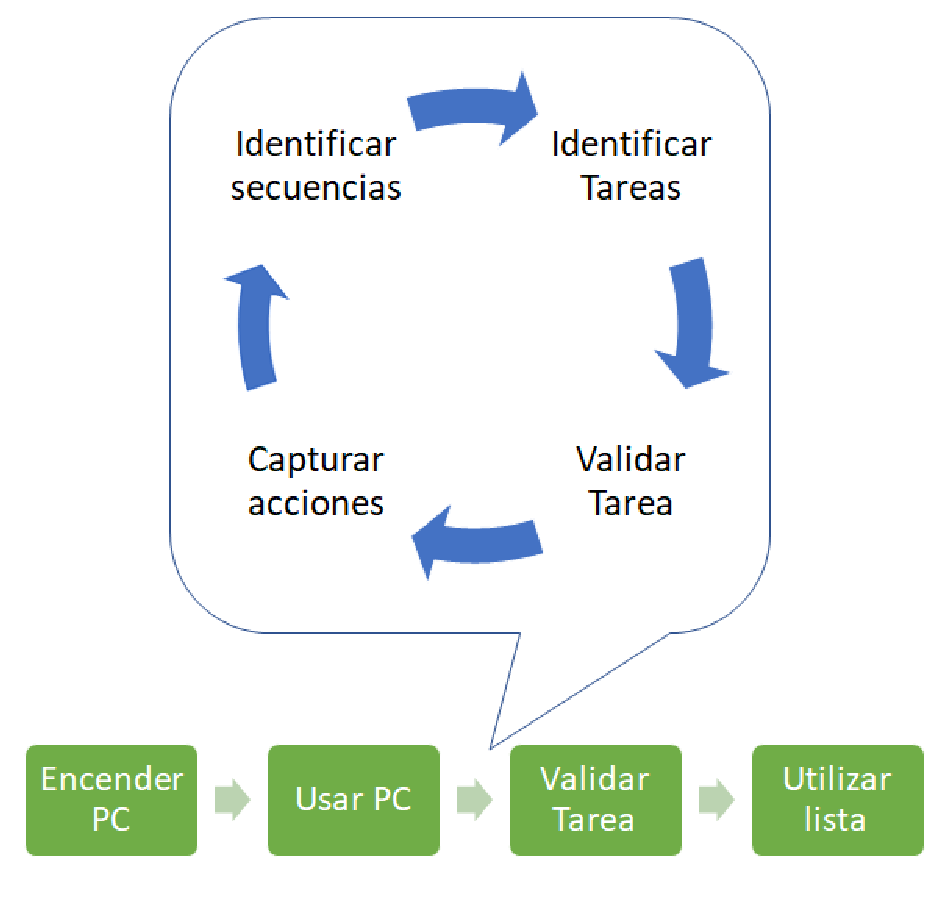
\includegraphics[width=0.6 \columnwidth]{Imagenes/Funcionamiento.eps}
\caption{Diagrama de funcionamiento.}
\label{fig:funcionamento}
\end{figure}
\end{frame}


\begin{frame}
\frametitle{Desarrollo}
\begin{figure}[h]
\centering
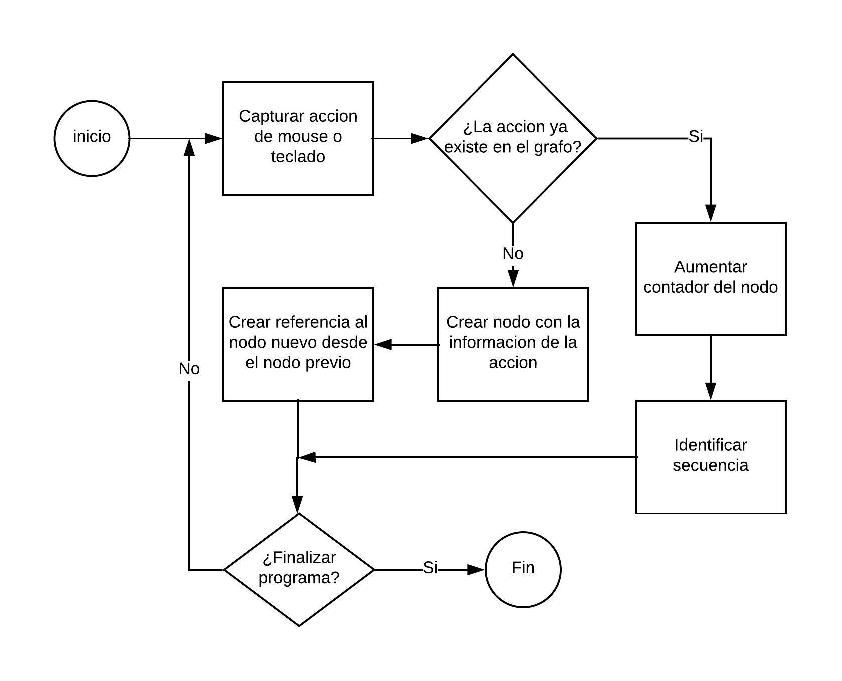
\includegraphics[height=0.55 \columnwidth]{Imagenes/Concepto1.eps}
\caption{Diagrama de flujo parte 1.}
\label{fig:bloques}
\end{figure}
\end{frame}

\begin{frame}
\frametitle{Desarrollo}
\begin{figure}[h]
\centering
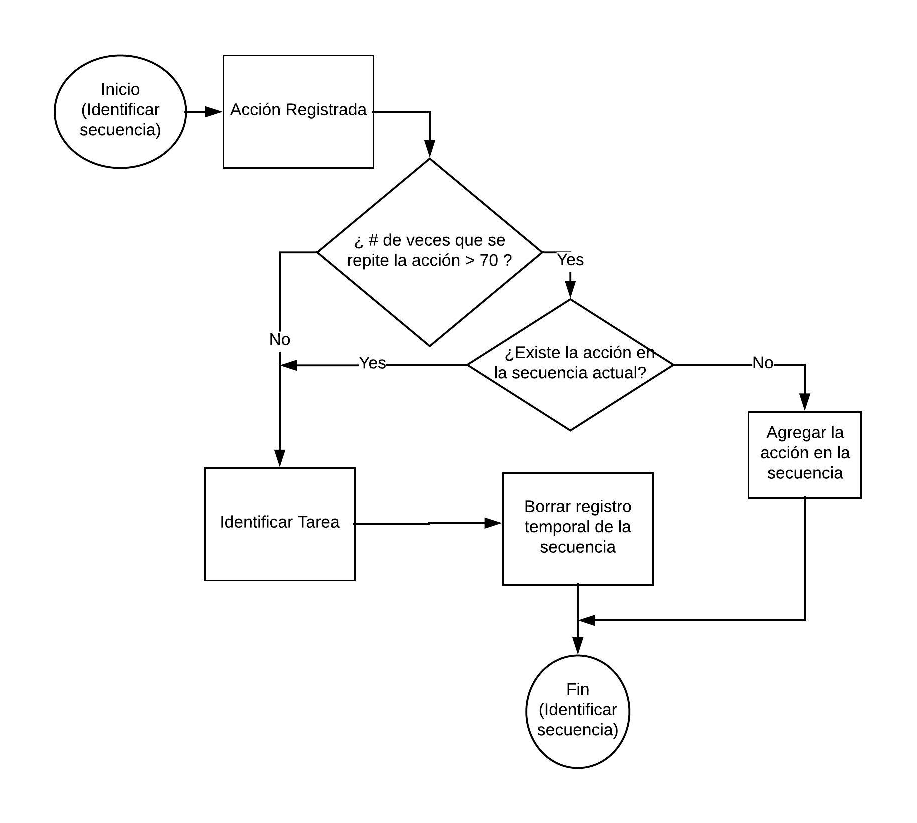
\includegraphics[height=0.55 \columnwidth]{Imagenes/Concepto2.eps}
\caption{Diagrama de flujo parte 2.}
\label{fig:bloques}
\end{figure}
\end{frame}

\begin{frame}
\frametitle{Desarrollo}
\begin{figure}[h]
\centering
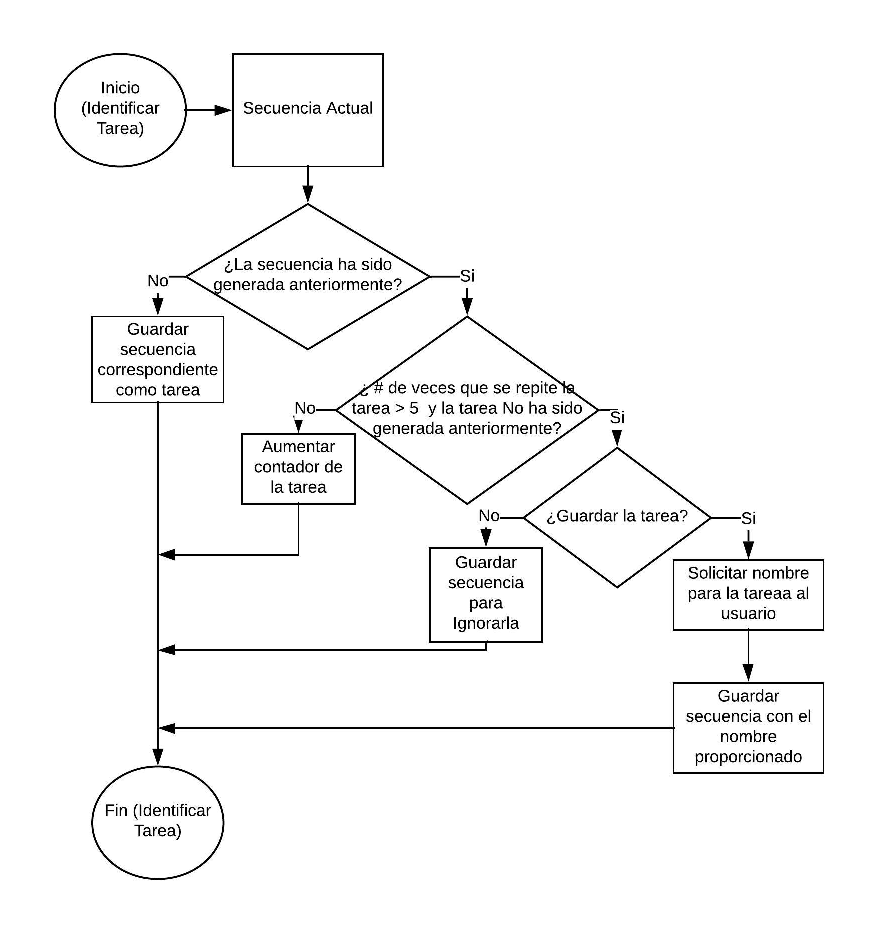
\includegraphics[height=0.55 \columnwidth]{Imagenes/Concepto3.eps}
\caption{Diagrama de flujo parte 3.}
\label{fig:bloques}
\end{figure}
\end{frame}


\begin{frame}
\frametitle{Interfaz Grafica}

\begin{figure}[H]
\centering
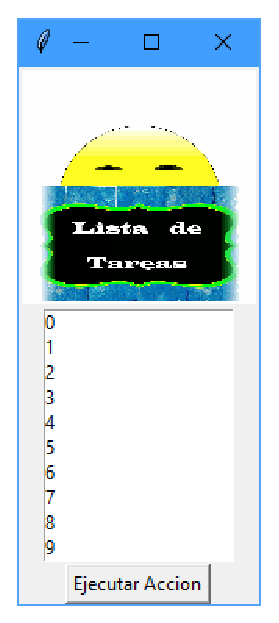
\includegraphics[width=0.2\columnwidth]{Imagenes/ventana1.eps}
\caption{Ventana principal con el asistente y una lista de tareas
 guardadas.}
\label{fig:v01}
\end{figure} 

\end{frame}


\begin{frame}
\frametitle{Interfaz Grafica}

\begin{figure}[H]
\centering
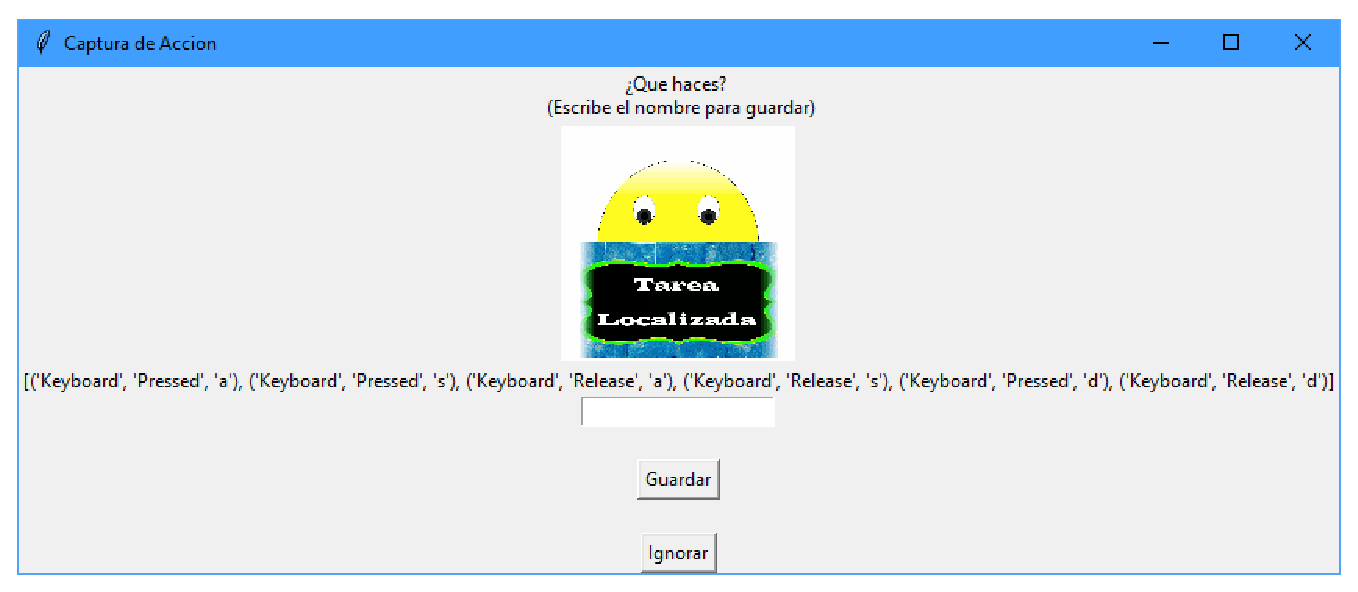
\includegraphics[width=1.0\columnwidth]{Imagenes/ventana2.eps}
\caption{Ventana mostrando una tarea encontrada.}
\label{fig:v02}
\end{figure}

\end{frame}
